\documentclass[svgnames,11pt]{beamer}
\input{/home/tof/Documents/Cozy/latex-include/preambule_commun.tex}
\input{/home/tof/Documents/Cozy/latex-include/preambule_beamer.tex}
%\usepackage{pgfpages} \setbeameroption{show notes on second screen=left}
\author[]{Christophe Viroulaud}
\title{Missile Patriot \\Nombres flottants}
\date{\framebox{\textbf{DonRep 04}}}
%\logo{}
\institute{Première - NSI}

\begin{document}
\begin{frame}
    \titlepage
\end{frame}
\begin{frame}
    \frametitle{}

    Le 25 février 1991, à Dharan en Arabie Saoudite, un missile Patriot (figure \ref{patriot}) américain a raté l’interception d’un missile Scud irakien. Ce dernier provoqua la mort de 28 personnes. La commission d'enquête a conclu à un défaut de l'horloge interne du missile. Cette dernière mesurait le temps en~1/10s.
    \begin{center}
        \centering
        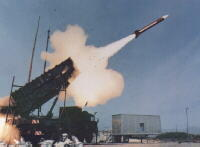
\includegraphics[width=5cm]{ressources/patriot.jpg}
        \captionof{figure}{Missile Patriot}
        \label{patriot}
    \end{center}

\end{frame}
\begin{frame}
    \frametitle{}

    \begin{center}
        \begin{framed}
            \centering Pourquoi la représentation en mémoire du temps a engendré cette erreur?
        \end{framed}
    \end{center}

\end{frame}
\section{Représentation générale des nombres réels}
\subsection{Écriture scientifique}
\begin{frame}
    \frametitle{Écriture scientifique}

    L'écriture scientifique des nombres réels répond à certaines règles:
    \begin{itemize}
        \item $1468=+1,468×10^3$
        \item $-891=-8,91×10^2$
        \item $0,00023=2,3×10^{-4}$
    \end{itemize}

\end{frame}
\begin{frame}
    \frametitle{}

    \begin{aretenir}[]
        La forme générale d'un nombre réel s'écrit:
        $$\pm 1×mantisse×10^{exposant}$$
    \end{aretenir}

\end{frame}
\subsection{Représentation en mémoire}
\begin{frame}
    \frametitle{Représentation en mémoire}

    La représentation des nombres réels en mémoire s'appuie sur l'écriture scientifique mais:
    \begin{itemize}
        \item elle utilise la \emph{base 2},
        \item l'exposant est \emph{biaisé} (décalé) d'une valeur \emph{d} dépendante du format (32 ou 64 bits),
        \item la mantisse est comprise entre [1;2[.
    \end{itemize}

\end{frame}
\begin{frame}
    \frametitle{}

    \begin{aretenir}[]
        La forme générale d'un nombre réel en mémoire s'écrit:
        $$(-1)^s×m×2^{n-d}$$
    \end{aretenir}

\end{frame}
\section{La norme \emph{IEEE 754}}
\subsection{Les choix effectués}
\begin{frame}
    \frametitle{Les choix effectués}

    C'est une norme mise au point par le \emph{Institute of Electrical and Electronics Engineers}. Des choix techniques ont été pris:
    \begin{itemize}
        \item Cette représentation n'utilise pas le \emph{complément à 2} pour stocker les exposants négatifs, mais un décalage d'une valeur \emph{d}.
        \item La mantisse est un nombre de la forme 1,xxxxxx. Afin de gagner 1 bit en précision, on ne représente que les chiffres après la virgule.
    \end{itemize}

\end{frame}
\subsection{Les formats}
\begin{frame}
    \frametitle{Les formats}

    \textbf{Simple précision:} Le nombre est représenté sur 32 bits.
    \begin{center}
        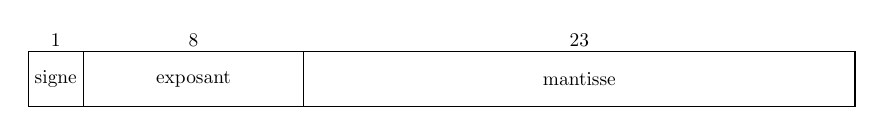
\begin{tikzpicture}[scale=0.7, transform shape]
            \draw (0,0) rectangle (1,1);
            \draw (0.5,0.5) node {signe} ;
            \draw (0.5,1.2) node {1} ;
            \draw (1,0) rectangle (5,1);
            \draw (3,0.5) node {exposant} ;
            \draw (3,1.2) node {8} ;
            \draw (5,0) rectangle (15,1);
            \draw (10,0.5) node {mantisse} ;
            \draw (10,1.2) node {23} ;
        \end{tikzpicture}
    \end{center}
    L'exposant est représenté sur 8 bits donc des entiers entre 0 et 255. Il est décalé de \emph{d=127} donc il est possible de représenter des exposants \emph{signés} dans l'intervalle [-127;128].
\end{frame}
\begin{frame}
    \frametitle{}

    \textbf{Double précision:} Le nombre est représenté sur 64 bits.
    \begin{center}
        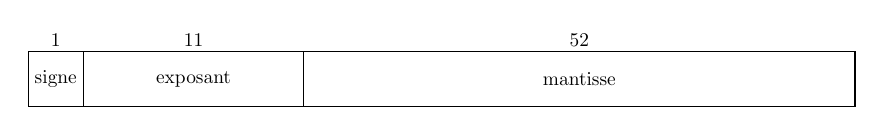
\begin{tikzpicture}[scale=0.7, transform shape]
            \draw (0,0) rectangle (1,1);
            \draw (0.5,0.5) node {signe} ;
            \draw (0.5,1.2) node {1} ;
            \draw (1,0) rectangle (5,1);
            \draw (3,0.5) node {exposant} ;
            \draw (3,1.2) node {11} ;
            \draw (5,0) rectangle (15,1);
            \draw (10,0.5) node {mantisse} ;
            \draw (10,1.2) node {52} ;
        \end{tikzpicture}
    \end{center}

\end{frame}
\begin{frame}
    \frametitle{}

    \begin{activite}
        \begin{enumerate}
            \item En s'appuyant sur le format 32 bits, donner la valeur du décalage \emph{d} pour le format 64 bits.
            \item En déduire les valeurs possibles pour l'exposant.
        \end{enumerate}
    \end{activite}

\end{frame}
\begin{frame}
    \frametitle{Correction}
\begin{itemize}
    \item $2^{11} = 2048$ donc entre 0 et 2047 nombres
    \item $d = 2^{11-1}-1=1023$ donc les exposants signés sont dans l'intervalle [-1023; 1024]
\end{itemize}
\end{frame}
\subsection{Un exemple}
\begin{frame}
    \frametitle{Un exemple}
    Considérons le mot de 32 bits:
    $$\overbrace{1}^{signe}\overbrace{10000110}^{exposant}\overbrace{10101101100000000000000}^{mantisse}$$
    

\end{frame}
\begin{frame}
    \frametitle{}

    \begin{itemize}
        \item signe: $(-1)^1=-1$
        \item mantisse: $1+2^{-1}+2^{-3}+2^{-5}+2^{-6}+2^{-8}+2^{-9} = 1,677734375$
        \item exposant: $(2^7+2^2+2^1)-127=134-127=7$
        \end{itemize}
        Le nombre représenté est:
        $$-1×1,677734375×2^7=-214,75$$
\end{frame}
\subsection{Pour aller plus loin}
\begin{frame}
    \frametitle{Pour aller plus loin}

    La norme \emph{IEEE 754} contient davantage de subtilités (représentation de 0, infini, dépassement de capacité, écart minimal...). Cette notion n'est pas au programme mais il peut être intéressant de lire la page Wikipédia correspondante:
\begin{center}
\url{https://fr.wikipedia.org/wiki/IEEE_754}
\end{center} 

\end{frame}
\section{Limites de la représentation}
\subsection{Convertir un nombre réel}
\begin{frame}
    \frametitle{Convertir un nombre réel}

    Pour donner la représentation de 0,6875, il faut d'abord convertir 0,6875 en base 2
    \begin{itemize}
        \item $0,6875×2 = 1,375$
        \item $0,375×2=0,75$
        \item $0,75×2=1,5$
        \item $0,5×2=1,0$
    \end{itemize}
$$0,6875_{10}=0,1011_2$$
\end{frame}
\begin{frame}
    \frametitle{Représentation en simple précision}

    {\LARGE$$0,1011_2=1,011×2^{-1}$$}
    \begin{itemize}
        \item signe: 0
        \item mantisse: 011000\dots
        \item exposant: $-1+127=126_{10}=01111110_2$
    \end{itemize}
    \bigskip
    $$\overbrace{0}^{signe}\overbrace{01111110}^{exposant}\overbrace{01100000000000000000000}^{mantisse}$$
\end{frame}
\subsection{Erreur de calcul?}
\begin{frame}[fragile]
    \frametitle{Erreur de calcul?}

\begin{center}
\begin{lstlisting}[language=Python , basicstyle=\ttfamily\small, xleftmargin=2em, xrightmargin=2em]
>>> 0.2 + 0.1
0.30000000000000004
\end{lstlisting}
\captionof{code}{Ce code renvoie un résultat surprenant.
}
\label{CODE}
\end{center}

\end{frame}
\begin{frame}
    \frametitle{}

    \begin{activite}
        \begin{enumerate}
        \item Convertir 0,2 en base 2.
        \item Que peut-on en déduire sur la représentation de ce nombre en mémoire?
        \end{enumerate}
        \end{activite}

\end{frame}
\begin{frame}
    \frametitle{Correction}

    Convertir 0,2 en représentation binaire:
    \begin{itemize}
        \item $0,2×2 = 0,4$
        \item $0,4×2=0,8$
        \item $0,8×2=1,6$
        \item $0,6×2=1,2$
        \item $0,2×2 = 0,4$
        \item \dots
    \end{itemize}
\begin{aretenir}[]
La représentation en mémoire de certains réels n'est pas exacte. Elle est tronquée en fonction de la taille du mot mémoire.
\end{aretenir}
\end{frame}
\section{Imprécision du missile Patriot}
\begin{frame}
    \frametitle{Imprécision du missile Patriot}

    L’horloge interne du missile Patriot mesure le temps en 1/10s soit 0,1s. Pour obtenir le temps en seconde, le système multipliait ce nombre par 10 en utilisant un registre de 24 bits en virgule fixe. 

\end{frame}
\begin{frame}
    \frametitle{}

    \begin{activite}
        \begin{enumerate}
        \item Convertir 0,1 en base 2. Que constate-t-on?
        \end{enumerate}
        Le registre de 24 bits contenait $(0,00011001100110011001100)_2$ et induisait une erreur binaire de $(0,0000000000000000000000011001100...)_2$, soit approximativement 0,000000095s en notation décimale.
        \begin{enumerate}
            \setcounter{enumi}{1}
        \item Le missile était allumé depuis 100 heures. Calculer le décalage \emph{noté \varepsilon} entre l'horloge interne et le temps réel.
        \item Un missile Scud volait à la vitesse de $1676m.s^{-1}$. Calculer la distance parcourue par le missile pendant la durée \varepsilon.
        \end{enumerate}
    \end{activite}
\end{frame}
\begin{frame}
    \frametitle{Correction}
    Convertir 0,1 en représentation binaire:
    \begin{itemize}
        \item $0,1×2 = 0,2$
        \item $0,2×2 = 0,4$
        \item $0,4×2=0,8$
        \item $0,8×2=1,6$
        \item $0,6×2=1,2$
        \item $0,2×2 = 0,4$
        \item \dots
    \end{itemize}
La représentation en mémoire de 0,1 sera tronquée.

\end{frame}
\begin{frame}
    \frametitle{Correction}

    \begin{itemize}
        \item $0,000000095×100×3600×10=0,34s$
        \item $1676×0,34 = 569m$
    \end{itemize}

\end{frame}
\begin{frame}
    \frametitle{}

    \begin{aretenir}[]
    La représentation en mémoire des nombres réels peut être approximative. On veillera à éviter les comparaisons entre deux nombres réels dans un programme.
    \end{aretenir}

\end{frame}
\end{document}